\section{Evaluations}
\label{evaluation}

In this section, we show the results of experimental evaluation of decentralized search. We first give an overview of the datasets and introduce the experiment settings of our evaluations. The quality of approximated path generated by decentralized search is evaluated from two aspects, distance accuracy and path diversity, in \ref{eval_accuracy} and \ref{eval_diversity} respectively. We then show both overhead of index and online search in \ref{eval_overhead}. In the last, we study the scalability of our system in \ref{eval_scalability}.

\subsection{Datasets}
\label{eval_datasets}

\begin{table}
		\caption{Datasets}
		\vspace{2 mm}
		\label{table:datasets}
		\begin{threeparttable}
			\centering
			\begin{tabular}{c|cccc} \hline
				Dataset & Type & $|V_{wcc}|$ & $|E_{wcc}|$ & $\overline{\sigma}$ \\ \hline
				Wiki & Communication & 2.4M & 4.7M & 3.9 \\ 
				Skitter & Internet & 1.7M & 11.1M & 5.07 \\ 
				Livejournal & Social & 4.8M & 43.4M & 5.6 \\ 
				Hollywood & Collaboration & 1.1M & 56.3M & 3.83 \\ 
				Orkut & Social & 3M & 117M & 4.21 \\ 
				Sinaweibo & Social & 58.7M & 261.3M & 4.15 \\ 
				Webuk & Web & 39.3M & 796.4M & 7.45 \\ 
				Friendster & Social & 65M & 1.8B & 5.03 \\ \hline
			\end{tabular}
			\begin{tablenotes}
				\item Datasets with number of vertices and edges in the largest weakly connected components, and average shortest distance $\overline{\sigma}$ of 100,000 vertex pairs.
			\end{tablenotes}
		\end{threeparttable}
\end{table}

We evaluate our algorithm on 8 graphs from different disciplines as shown in table \ref{table:datasets} in ascending order on the number of edges. All graphs are complex networks that have power-law degree distribution and relatively small diameter. All datasets have at least millions of edges, the largest one has almost two billion edges. To simplify our experiments, we treat each graph as undirected, un-weighted graphs. We only use the largest weakly connected component of each graph which consist of more than $90\%$ of vertices for all graphs. All datasets are collected from \cite{snapnets} and \cite{nr}.

\subsection{System settings}
\label{eval_system}

We evaluate our algorithms in both distributed settings and centralized settings.
%For distributed settings, we use 20 Cloudlab ~\cite{RicciEide:login14} r320 nodes from Apt cluster. Each node has a 8-core 2.1GHz Xeon E5-2450 processor and 16 GB memory. All the experimental traffics are carried on a 10Gbps Ethernet. 
For distributed settings, we use 20 Amazon EC2 m4.xlarge virtual machines. Each virtual machine has 4 vCPUs and 16 GB memory. We also implemented a centralized version on a Cloudlab~\cite{RicciEide:login14} c8220 server with two 10-core 2.2GHz E5-2660 processors and 256GB memory. Powergraph~\cite{180251} is the platform for distributed version and ~Snap~\cite{snapnets} is the platform for centralized version. All algorithms are implemented in C++. 

All the evaluations use the same landmark selection strategy, a variation based on $DEGREE/h$ strategy from reference~\cite{Potamias:2009:FSP:1645953.1646063} which take both vertex degree and distance to existing landmarks into consideration. On selecting a new landmark, each vertex receive a rank which is the product of its degree and the sum of distance to all the existing landmarks. The vertex with highest rank will be added to the landmark set. We denote number of landmarks as $k$.

Quries in our experiments are randomly generated. For accuracy evaluations, since performing BFS on large graphs in our datasets is extremely slow, to control the number of exact pairs of shortest path distance we need to find using BFS, we randomly choose 1,000 vertices of each graph as source vertices. For each source vertex, we then randomly choose 100 vertices as target vertices. We are able to generate 100,000 queries with 1000 BFS. All results in \ref{eval_accuracy} are averaged among 100,000 queries.

\subsection{Approximation Accuracy}
\label{eval_accuracy}

\begin{figure*}[t]
    \centering
    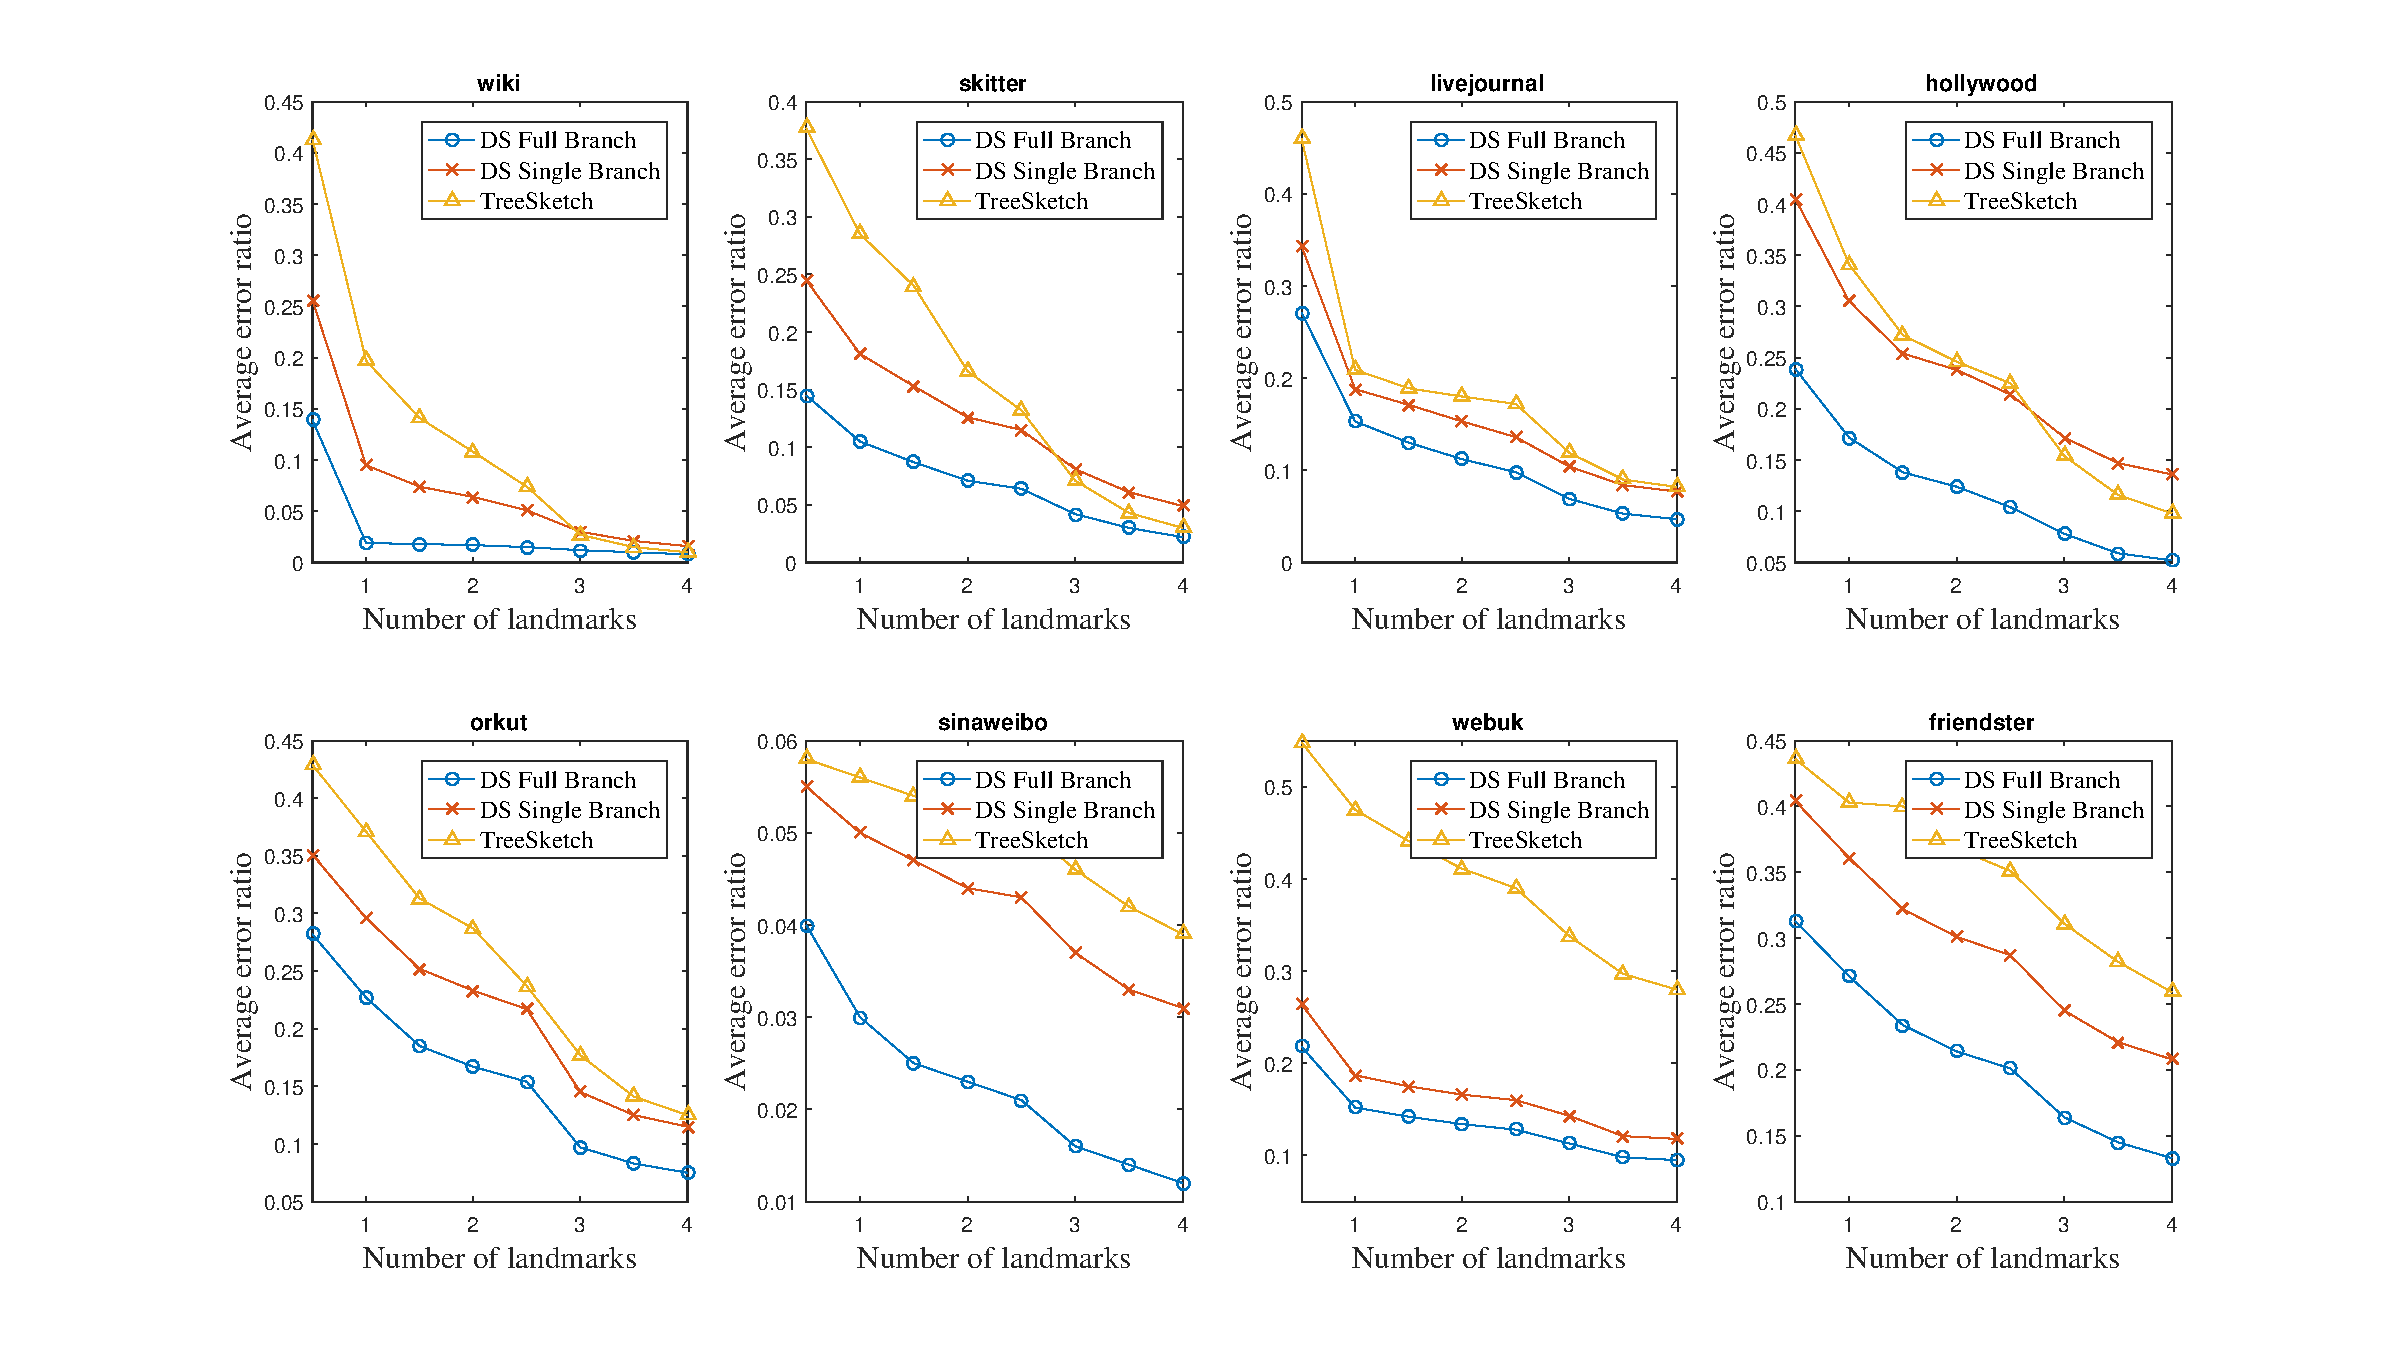
\includegraphics[width=\linewidth]{./figures/accuracy_stepy.pdf}
    \caption{The accuracy of the approximated distance of decentralized search and various optimizations compared to TreeSketch.}
    \label{fig:accuracy_stepy}
\end{figure*}

We first evaluate the approximation accuracy of decentralized search. We use the average approximation error as the measure of accuracy which is defined as follows:
\[
E_{p_{appr.}(s,t)} = \frac{|p_{appr.}(s,t)| - d_G(s,t)}{d_G(s,t)}
\]
We show the results of 4 variants of decentralized search with mixture of different tie strategy and index construction approach. All the decentralized search are performed with bidirectional search. We also list the performance of an state-of-the-art existing method, TreeSketch, from reference~\cite{Gubichev:2010:FAE:1871437.1871503}. [Reference~\cite{6399472} also includes a online search method but is quite similar to TreeSketch in nature so that we haven't included here.] We perform all 5 approaches for 100,000 queries under various size of landmark sets and show the averaged results in Fig. \ref{fig:accuracy_stepy}.

We can see in Fig. \ref{fig:accuracy_stepy} that decentralized search achieves better accuracy in most of cases. Especially with small landmark sets, i.e. $k < 5$, decentralized search outperforms TreeSketch on all the graphs. And Full branch decentralized search outperforms TreeSketch with any landmark sets on all eight graphs. When the search are carried on the index constructed by our greedy heuristic, the performance gain is much noticeable, with 1.76 to 8.09 times lower average error ratio for 1 landmark and 1.25 to 2.59 times lower average error ratio for 20 landmarks on various graphs.

For tie breaking strategies, full branch tie strategy always outperforms single branch tie strategy with large margins as it explores more vertices, that of course, comes with larger search overheads that will be discussed in \ref{eval_overhead}. The average error ratio of full branch is lower than 1.21 to 1.84 times of single branch with 1 landmark and 1.24 to 2.61 times with 20 landmarks on various graphs. As the number of landmark increases, the performance gain also increase. The single branch and full branch set the accuracy range that is achievable by Decentralized search.  

Decentralized search carried on index constructed by greedy heuristic has much lower error ratio than decentralized search with regular index. The average error ratio of decentralized search is 1.17 to 2.51 times lower for single branch and 1.27 to 2.73 times lower for full branch for 1 landmark than decentralized search based on regular index. For higher landmark size, regular index actually outperforms index constructed by greedy heuristic in some cases, the reason should be that the greedy heuristic may introduce higher redundancy, i.e. multiple landmark generate similar index due to same goal, when number of landmark increases. The ratio ranging from 0.77 to 1.41 for single branch and 0.57 to 1.33 for full branch under 20 landmarks.

\subsection{Path Diversity}
\label{eval_diversity}

\begin{table}
	\caption{Path diversity (k = 2)}
    \label{table:pdiv}
    \centering
    \begin{tabular}{c|ccc} \hline
				Graph&Path cnt(DS)&Path cnt(TS)&Out ratio \\ \hline
				Wiki&28.9&1.9&0.372 \\ 
				Skitter&24.1&2.4&0.418 \\ 
				Livejournal&30.8&1.9&0.338 \\ 
				Hollywood&9.9&2.6&0.471 \\ 
				Orkut&19.2&3.2&0.465 \\ 
				Sinaweibo&32.0&3.0&0.301 \\ 
				Webuk&704.1&2.0&0.501 \\ 
				Friendster&16.8&2.8&0.39 \\ \hline
    \end{tabular}
\end{table}

We evaluate the path diversity of paths returned by decentralized search in this section. By forking the search into multiple search during tie breaking, the algorithm can return various paths with same length, i.e. the estimated shortest distance between two vertices. Note that only paths with estimated shortest distance are recorded, longer paths are disgarded. Table \ref{table:pdiv} shows average number pf paths returned by decentralized search with full branch tie strategies and TreeSketch. The average path count of full branch decentralized search is significant higher than that of TreeSketch, from 3.73 to 345.13 times for various graphs. 

Moreover, not only full branch decentralized search return higher number of paths, but the returned paths are also not constrained by the label of source and target vertices like TreeSketch do, i.e., paths found by TreeSketch only contain vertices in labels of source and target vertex. We define the out ratio of a path longer than 1 hop as follow:
\[
Out\_ratio(p(s,t)) = \frac{|\{u:u \in p(s,t), u \notin L(s) \cup L(t)\}|}{|p(s,t)| - 2}
\]
It shows the degree of a path relying on the labels of source and target vertex. The higher the value, the lower the dependence. The average out ratio for full branch decentralized search on various graphs ranges from 0.301 to 0.501.

\subsection{Overhead}
\label{eval_overhead}

\begin{table}
		\caption{Index overhead per landmark}
    \label{table:ioh}
    \centering
    \begin{tabular}{c|cc} \hline
				Graph&Index size(MB)&Index time(s)\\ \hline
				Wiki&189.9&0.8 \\ 
				Skitter&143.7&2.8 \\ 
				Livejournal&429.4&8.7 \\ 
				Hollywood&84.1&8 \\ 
				Orkut&246.3&20.7 \\ 
				Sinaweibo&4313.8&87.3 \\ 
				Webuk&4068.9&73.9 \\ 
				Friendster&5497.7&348.6 \\ \hline
    \end{tabular}
\end{table}

The index overhead is shown in table \ref{table:ioh}. In our implementation, the index of each vertex is stored as vector of C++ standard library. And each vertex id is represented by 8-byte unsigned long. The size shown in table \ref{table:ioh} is the sum of vector size of each vertex. 

\begin{figure*}[t]
    \centering
    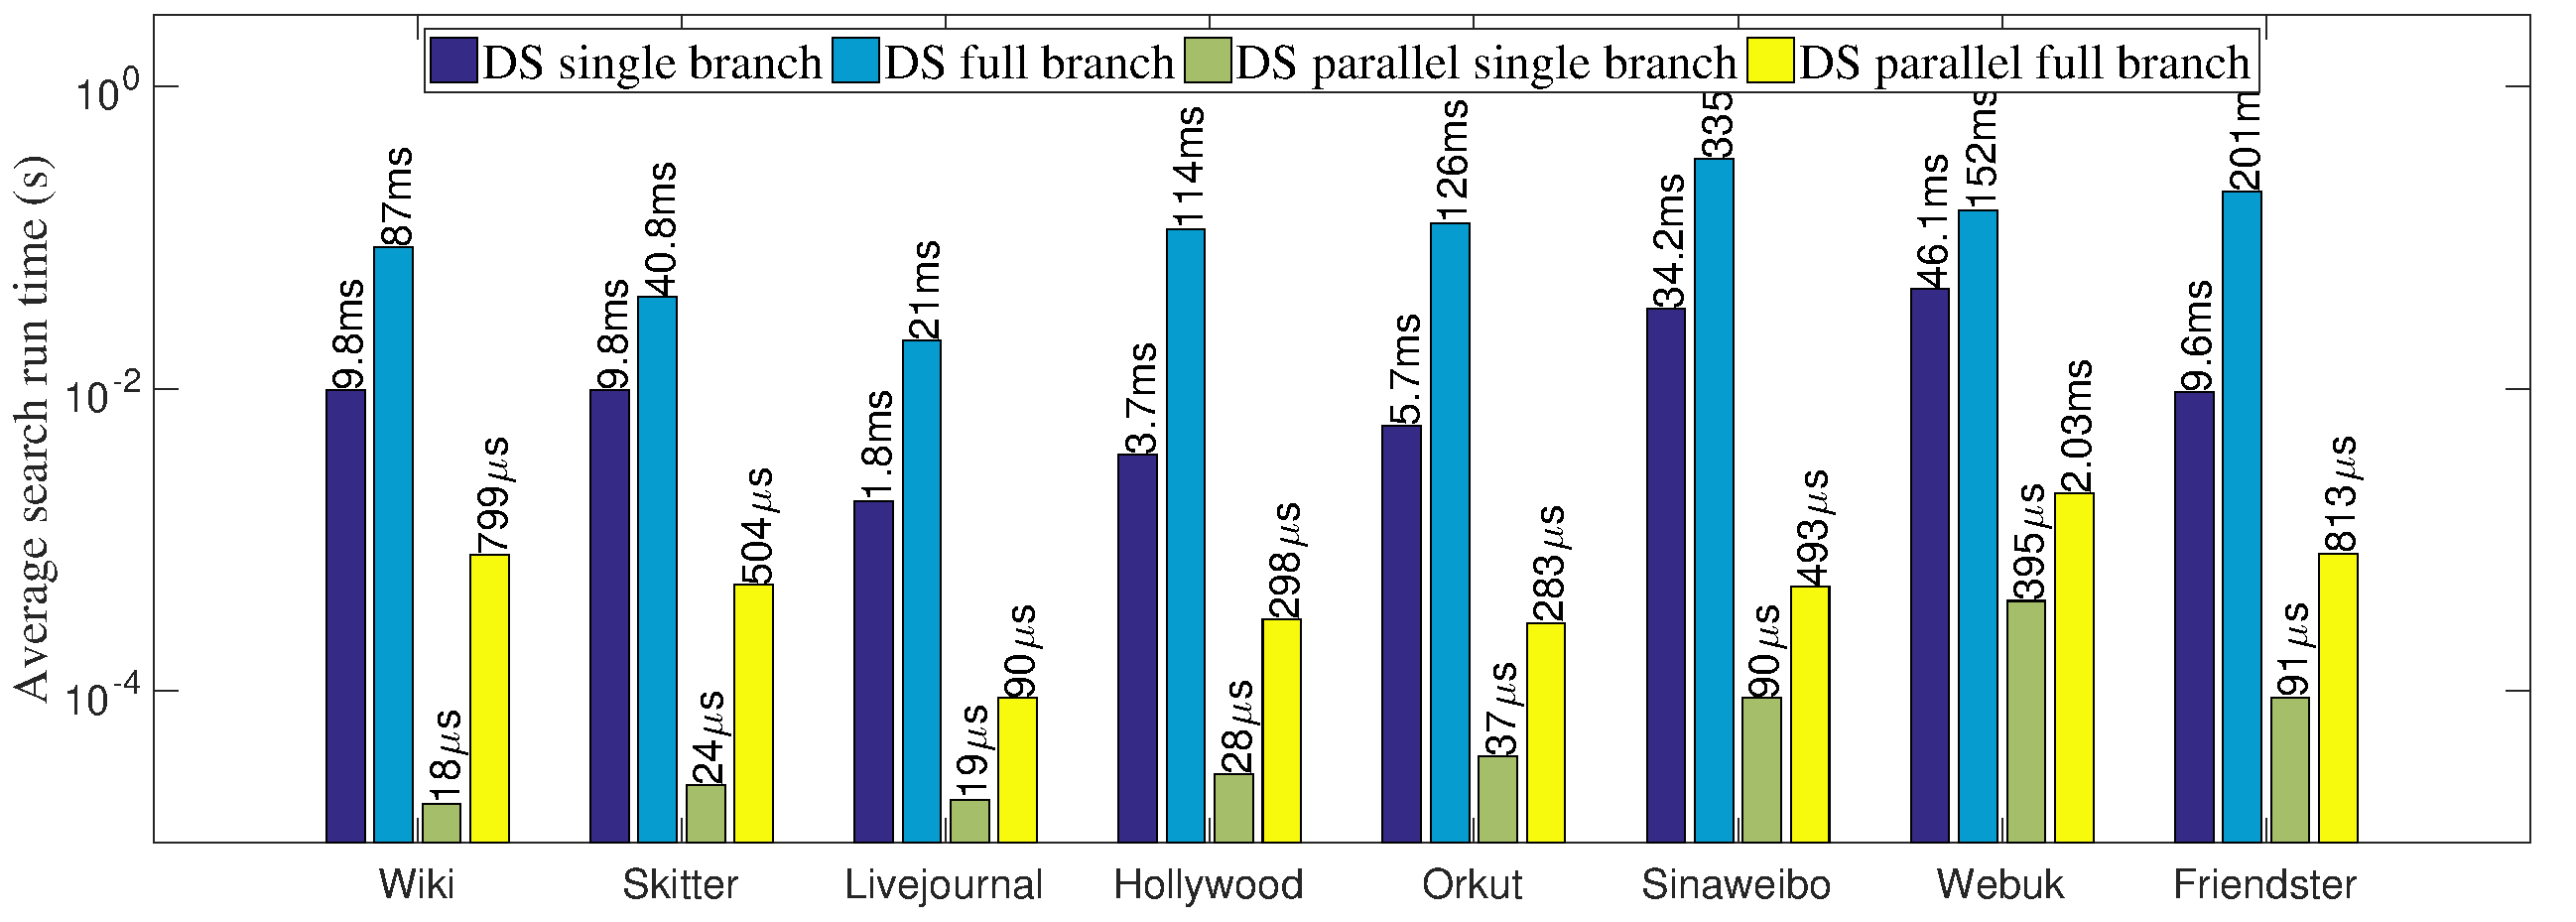
\includegraphics[width=\linewidth]{./figures/overhead_search.pdf}
    \caption{The average search time of decentralized search with various optimizations.}
    \label{fig:overhead_search}
\end{figure*}

Fig. \ref{fig:overhead_search} shows the online search overhead in log scale for both non-parallel mode and parallel batch mode. [add treesketch data later] By examing all the neighbors of a vertex at each step, decentralized search introduces much higher online search overhead than TreeSketch. Nevertheless, due to that decentralized search has very low foot print, large amount of searches can run independently in parallel efficiently. We can see in Fig. \ref{fig:overhead_search}, the batch mode perform 100,000 queries simultaneously, which lead to very low average search time for each query. The search time is reduced to from 0.18\% to 1.1\% for single branch and from 0.15\% to 1.3\% for full branch compared to non-parallel mode. 

For both non-parallel and parallel mode, full branch tie break strategy introduces much higher overhead than single branch strategy. Ranging from 3.3 to 30.8 times higher search time for non-parallel version and from 5.1 to 44.4 times higher average search time for parallel version.

[search memory overhead]

[search time to graph stat analysis]

\subsection{Scalability}
\label{eval_scalability}

Since our algorithm is designed for large-scale networks, scalability is another major concern of our algorithm. Due to that we implement the algorithm in a distributed setting and execute queries in a parallel way, we study how our algorithm performs when number of machines and queries increase. We only perform single branch decentralized search here as full branch search is equal to multiple single branch searches.

\begin{figure}[t]
    \centering
    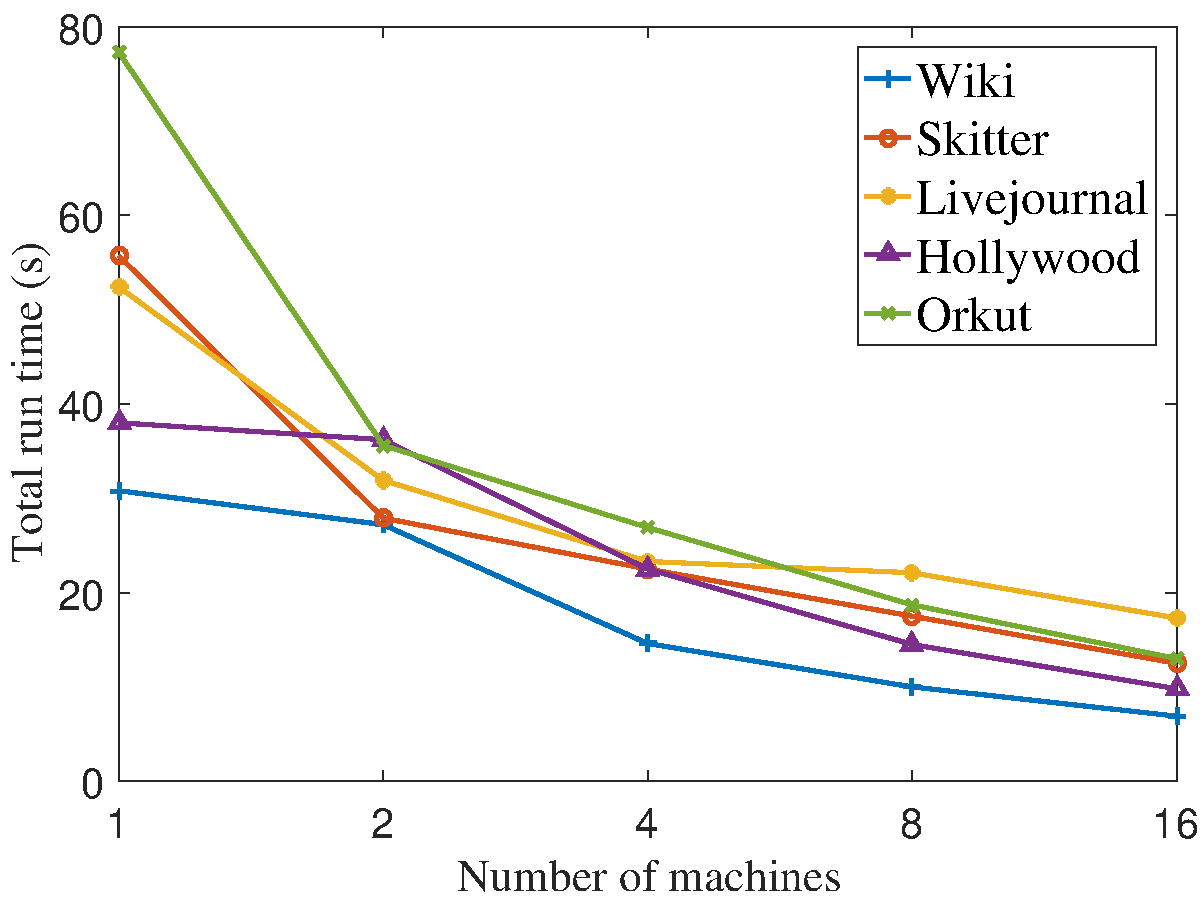
\includegraphics[width=\linewidth]{./figures/scale_machine.pdf}
    \caption{The average search time as the number of machines increase}
    \label{fig:scale_machine}
\end{figure}

We first evaluate the search time when number of machines increasing. Results shown in Fig. \ref{fig:scale_machine} are averaged over 1,000,000 queries. We can see the trend is that the average run-time decreases as the number of machines increase. The average search time decreases fast when small number of machines are deployed and slow down when large number of machines are used. The total run time on 16 machines range from 0.17 to 0.33 of the total run time on a single machine for various graphs.

[use the strong scaling figure here?]

\begin{figure}[t]
    \centering
    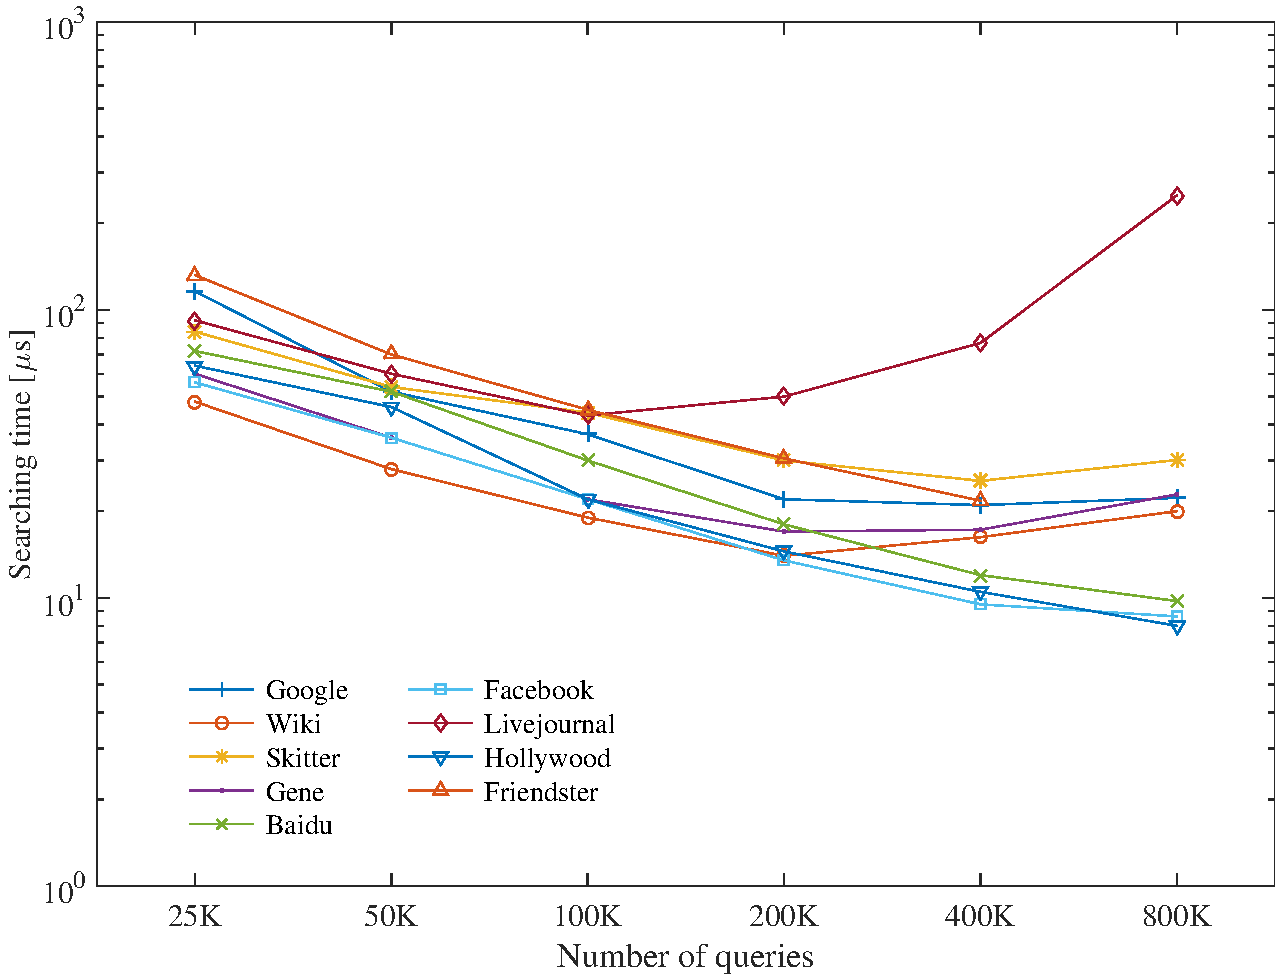
\includegraphics[width=\linewidth]{./figures/scale_query.pdf}
    \caption{The average search time as the number of queries increase}
    \label{fig:scale_query}
\end{figure}

We observe great scalability of decentralized search as number of queries increase. All experiments are carried on 20 machines in this section. We can see in Fig. \ref{fig:scale_query} that the average search time quickly goes down when the number of queries is small. Because for small number of queries, constant overheads such as engine start/stop is the major part of run time. For large number of queries, the average run time still keep dropping. The growth of total search time never catch up with the growth of number of queries until it reaches the system limit, i.e. memory limit or network limit.

%\begin{figure}[t]
    %\centering
    %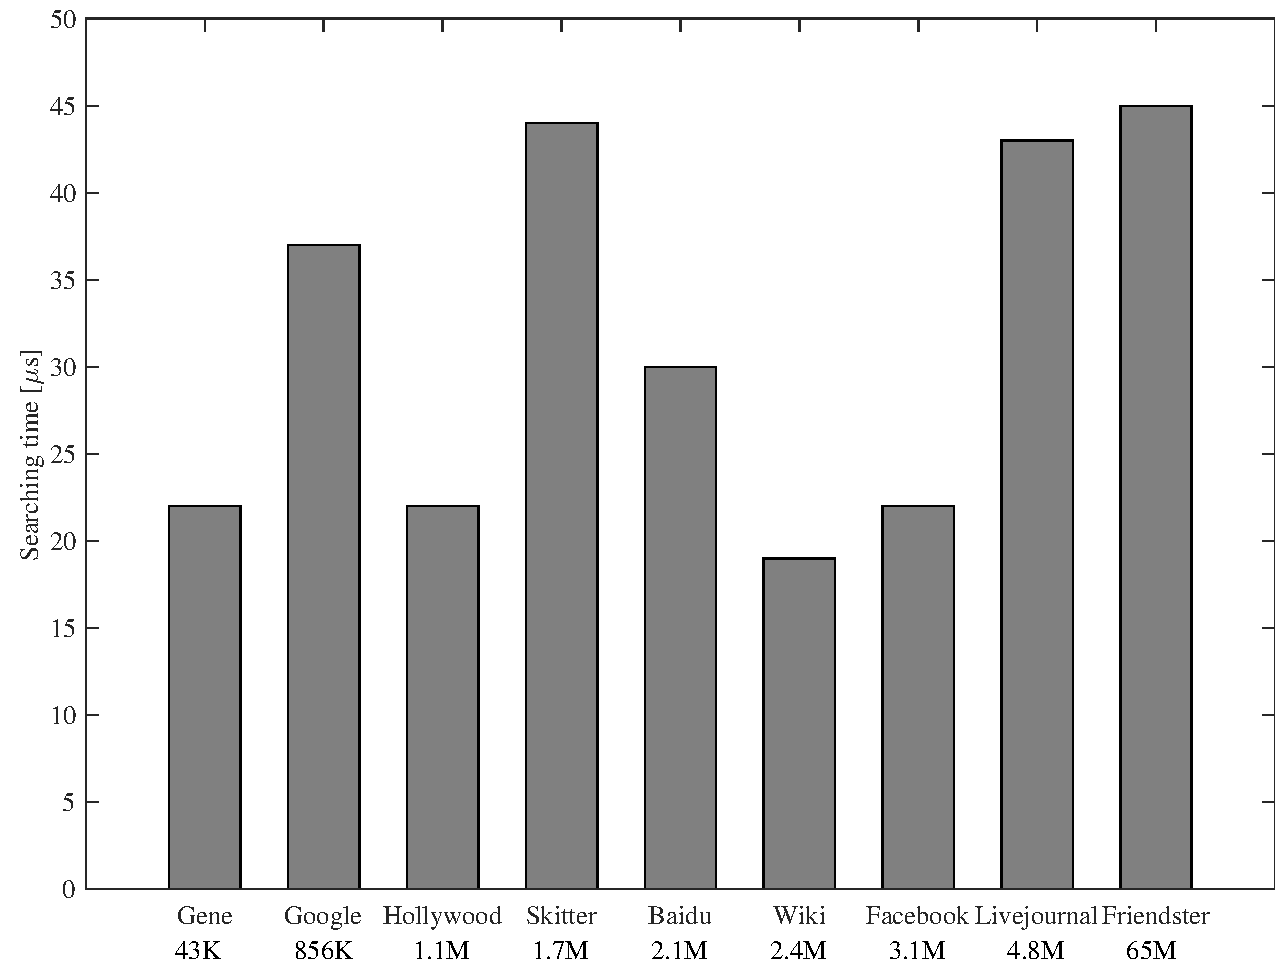
\includegraphics[width=\linewidth]{./figures/scale_graph.pdf}
    %\caption{The average search time for different size of graphs}
    %\label{fig:scale_graph}
%\end{figure}
%
%In the last experiment, we evaluate the search time as the size of graph increases. Unlike BFS which needs to traverse neighbors of $O(n)$ vertices, decentralized search only needs to exam neighbors of $O(log(n))$ vertices for complex networks due to the small world property. We can clearly see in Fig. \ref{fig:scale_graph} that as the number of vertices increases, average search time of decentralized search does not follow the same trend. The graph friendster which have sixty-five millions vertices have average search time only $2.05$ times more than graph mouse-gene which only have forty-three thousand vertices.

%\subsection{error distribution}
%
%\begin{figure}[t]
    %\centering
    %\includegraphics[width=\linewidth]{./figures/empty.pdf}
    %\caption{Distribution of errors of different length}
    %\label{fig:distribution}
%\end{figure}
%
%\comment{we want to show that the algorithm performs equally well for various path length}
%In the last, we study the error distribution according to the length of exact shortest path.
